% signaling_pathway.tex - 信号通路与分子机制图模板 (Cellular Signaling Pathway)
% 编译方式: pdflatex signaling_pathway.tex 或 xelatex signaling_pathway.tex
\documentclass[tikz,border=10pt]{standalone}
\usepackage{xcolor}
\usepackage{tikz}
\usetikzlibrary{arrows.meta, positioning, calc, shapes.geometric, backgrounds, decorations.pathmorphing}

\definecolor{natureblue}{HTML}{4E79A7}
\definecolor{natureorange}{HTML}{F28E2B}
\definecolor{naturered}{HTML}{E15759}
\definecolor{naturecyan}{HTML}{76B7B2}
\definecolor{naturegreen}{HTML}{59A14F}
\definecolor{darktext}{HTML}{262626}
\definecolor{subtext}{HTML}{64748B}
\definecolor{membranecolor}{HTML}{E2E8F0}
\definecolor{membraneborder}{HTML}{94A3B8}

\begin{document}
\sffamily
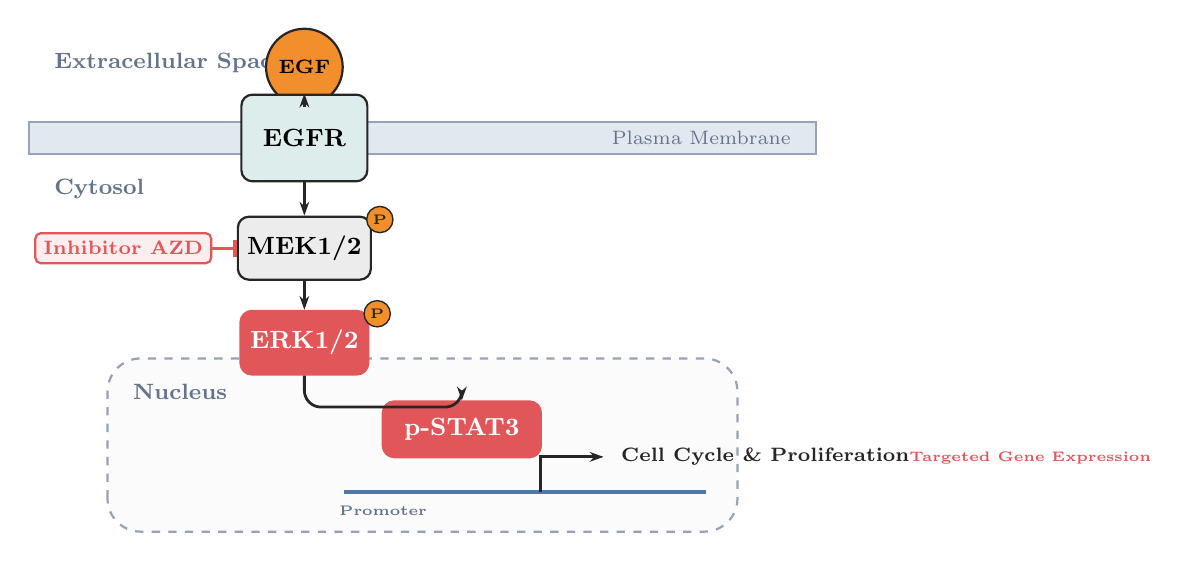
\begin{tikzpicture}[
    scale=1.0,
    protein/.style={
        rectangle,
        rounded corners=4pt,
        draw=darktext,
        line width=0.8pt,
        fill=natureblue!15,
        minimum width=1.6cm,
        minimum height=0.8cm,
        align=center,
        font=\small\bfseries
    },
    accentprotein/.style={
        protein,
        draw=naturered,
        fill=naturered,
        text=white,
        line width=1.0pt
    },
    inhibitor/.style={
        rectangle,
        rounded corners=2pt,
        draw=naturered,
        fill=naturered!10,
        text=naturered,
        line width=0.8pt,
        font=\scriptsize\bfseries,
        inner sep=3pt
    },
    actarrow/.style={
        -{Stealth[length=5pt,width=3.5pt]},
        line width=1.0pt,
        color=darktext
    },
    inhibarrow/.style={
        -{Bar[width=6pt]},
        line width=1.2pt,
        color=naturered
    },
    ptm/.style={
        circle,
        draw=darktext,
        fill=natureorange,
        inner sep=1.2pt,
        font=\tiny\bfseries,
        line width=0.5pt,
        text=darktext
    }
]

    % --- 1. 背景边界: 细胞膜与细胞核 ---
    % 细胞外文字
    \node[anchor=north west, font=\footnotesize\bfseries\color{subtext}] at (0.2, 5.8) {Extracellular Space};
    
    % 细胞膜 (双分子层风格)
    \draw[fill=membranecolor, draw=membraneborder, line width=0.8pt] (0, 4.4) rectangle (10, 4.8);
    \node[anchor=east, font=\scriptsize\color{subtext}] at (9.8, 4.6) {Plasma Membrane};

    % 胞质文字
    \node[anchor=north west, font=\footnotesize\bfseries\color{subtext}] at (0.2, 4.2) {Cytosol};

    % 细胞核边界 (双虚线)
    \draw[fill=gray!3, draw=membraneborder, dashed, line width=0.8pt, rounded corners=12pt] (1.0, -0.4) rectangle (9.0, 1.8);
    \node[anchor=north west, font=\footnotesize\bfseries\color{subtext}] at (1.2, 1.6) {Nucleus};

    % --- 2. 膜受体系统 (RTK) ---
    % 配体 (Ligand)
    \node[circle, draw=darktext, fill=natureorange, line width=0.8pt, minimum size=0.6cm, font=\scriptsize\bfseries] (ligand) at (3.5, 5.5) {EGF};
    
    % 跨膜受体 (Receptor Dimer)
    \node[protein, fill=naturecyan!25, minimum height=1.1cm] (receptor) at (3.5, 4.6) {EGFR};
    \draw[actarrow] (ligand) -- (receptor);

    % --- 3. 胞质激酶传导级联 ---
    % 激酶 1: RAS / RAF
    \node[protein, fill=gray!15] (kinase1) at (3.5, 3.2) {MEK1/2};
    \draw[actarrow] (receptor) -- (kinase1);
    \node[ptm] at ($(kinase1.north east)+(0.1, -0.05)$) {P};

    % 小分子抑制剂阻断
    \node[inhibitor] (drug) at (1.2, 3.2) {Inhibitor AZD};
    \draw[inhibarrow] (drug) -- (kinase1);

    % 核心突破激酶: ERK1/2 (高亮高饱和强调色)
    \node[accentprotein] (kinase2) at (3.5, 2.0) {ERK1/2};
    \draw[actarrow] (kinase1) -- (kinase2);
    \node[ptm] at ($(kinase2.north east)+(0.1, -0.05)$) {P};

    % --- 4. 易位入核与转录调控 ---
    % 核内转录因子
    \node[accentprotein, minimum width=2.0cm, minimum height=0.7cm] (tf) at (5.5, 0.9) {p-STAT3};
    \draw[actarrow, rounded corners=6pt] (kinase2.south) -- ++(0,-0.4) -| (tf.north);

    % DNA 双螺旋线
    \draw[line width=1.5pt, color=natureblue] (4.0, 0.1) -- (8.6, 0.1);
    \node[anchor=north, font=\tiny\bfseries\color{subtext}] at (4.5, 0.05) {Promoter};

    % 转录起始折线箭头 (TSS Bent Arrow)
    \draw[actarrow, line width=1.0pt] (6.5, 0.1) -- ++(0, 0.45) -- ++(0.8, 0);
    \node[anchor=west, font=\scriptsize\bfseries\color{darktext}] at (7.4, 0.55) {Cell Cycle \& Proliferation\\{\tiny\color{naturered}\bfseries Targeted Gene Expression}};

\end{tikzpicture}
\end{document}
